\documentclass[10pt]{article}

\usepackage[a4paper,margin=0.75in]{geometry}
\usepackage{amsmath,amssymb,amsthm}
\usepackage{array}
\usepackage{booktabs}
\usepackage{graphicx}
\usepackage{float}
\usepackage[hidelinks]{hyperref}
\hypersetup{
  pdftitle={Supplementary Information: Exact reversible choice coding with retrospective assay-guided selection},
  pdfsubject={Anonymous Bioinformatics methods manuscript supplementary information},
  pdfkeywords={DNA data storage, constrained coding, PCR efficiency, reversible coding}
}

\newcommand{\DNA}{\{A,C,G,T\}}
\newtheorem{proposition}{Proposition}
\renewcommand{\thefigure}{S\arabic{figure}}
\renewcommand{\thetable}{S\arabic{table}}
\emergencystretch=2em

\title{Supplementary Information for\\Exact reversible choice coding with retrospective assay-guided selection in PCR-tested oligonucleotide libraries}
\author{}
\date{}

\begin{document}
\maketitle

\section{Evidence contract}

The study has linked but non-interchangeable evidence layers. Bidirectional GCall/GCfix codebooks test retrospective measured cross-pool selection rather than a preregistered final lockbox. An outcome-blind KAPA codebook fixed by a dated analysis plan before local scoring tests the same source models in already-public measurements from an external laboratory reported within the same source publication; this is neither prospective preregistration nor independent third-party replication. A separate Q5 codebook is a secondary exploratory altered-protocol measured analysis. The generated-language layer tests whether the fixed-choice interface attaches to a total exact codec with an explicit rate cost and reports model-predicted scores only. Prospective synthesis and PCR of emitted codewords were not performed.

The supported claim is therefore that a frozen source-only assay score can choose among fixed-size exactly decodable representatives, has retrospective measured selection utility in PCR-tested libraries under matched conditions, and costs exactly one payload bit per selector bit in the generated 108-nt codec. Exact reversibility is independent of the score and assay; observed biological utility is assay-dependent. The study does not claim mechanism, independent replication, prospective emitted-codeword PCR, synthesis, sequencing, empirical recovery, achieved storage density, full weighted-language capacity or end-to-end storage superiority.

\begin{table}[H]
\centering
\scriptsize
\begin{tabular}{@{}p{0.11\linewidth}p{0.15\linewidth}p{0.14\linewidth}p{0.10\linewidth}p{0.14\linewidth}p{0.16\linewidth}@{}}
\toprule
Layer & Evidence type & Material & Outcome status & Supports & Does not support\\
\midrule
1 & Computational verification & Rank/unrank, modulo-$N$, 65,024 candidates & No assay & Exact language, fibers, inversion, failure paths & PCR or synthesis benefit\\
2 & Retrospective measured & GCall/GCfix codebooks & Previously measured & Within-fiber measured selection under source-study assay & Prospective emitted-codeword performance\\
3 & Same-publication external-laboratory & Analysis-plan-locked external KAPA codebook & Previously measured, already public & Matched-assay transfer to another laboratory pool & Independent third-party replication or prospective preregistration\\
4 & Altered-protocol measured & Exploratory external Q5 codebook & Previously measured & Assay-transfer boundary & Polymerase-universal quality\\
5 & Generated predicted & Generated exact-codec candidates & Predicted only & Rate--score and mapping diagnostics & Measured gain\\
6 & Prospective validation & Synthesis and PCR of emitted candidates & Not performed & Not available & Not claimed\\
\bottomrule
\end{tabular}
\caption{Evidence hierarchy used throughout the manuscript, figures and machine-readable outputs. ``Measured'' denotes an existing PCR measurement; it does not imply that the sequence was emitted by the present codec.}
\label{tab:s-evidence-hierarchy}
\end{table}

\section{Exact base coding and reversible choice}

\subsection{Exact completion counting}

For length $n=108$, define
\[
 \mathcal C=\{x\in\DNA^{108}:49\leq \operatorname{GC}(x)\leq59,
 \ \operatorname{HP}_{\max}(x)\leq3\}.
\]
The state after a prefix records position, GC count, last nucleotide and current homopolymer run. For state $q$ and $t$ remaining positions, let $C_t(q)$ be the number of legal terminal completions. Exact integer counts obey
\[
 C_0(q)=\mathbf 1\{q\text{ satisfies the final whole-sequence GC interval}\},\qquad
 C_t(q)=\sum_{a:\delta(q,a)\ \mathrm{legal}} C_{t-1}(\delta(q,a)).
\]

\begin{proposition}[Exact rank and unrank]
Lexicographic branch intervals with widths $C_{t-1}(\delta(q,a))$ partition $[0,C_t(q))$. Recursively selecting the interval containing a rank defines an unranker $E$, and summing the masses of earlier branches defines a ranker $D$, with $D(E(k))=k$ for every $0\leq k<C_n(q_0)$.
\end{proposition}

\begin{proof}
At $t=0$ the empty continuation has mass one exactly for an accepting state. Assume the statement for $t-1$. Continuations beginning with different legal nucleotides are disjoint, and the induction hypothesis gives each branch cardinality exactly. Their ordered cumulative masses therefore form contiguous, non-overlapping intervals whose union is $[0,C_t(q))$. Unranking chooses one interval, subtracts its left endpoint and recurses; ranking adds the preceding interval widths and applies the inverse recursion to the suffix. Exact integer arithmetic preserves the partition and the inverse at every depth.
\end{proof}

Top-down memoization and an independently implemented bottom-up recurrence returned the same total:
\[
\begin{aligned}
 |\mathcal C|={}&21{,}520{,}867{,}790{,}325{,}216{,}400{,}381{,}593{,}480{,}072{,}139{,}809{,}\\
 &549{,}357{,}542{,}204{,}871{,}770{,}858{,}223{,}072.
\end{aligned}
\]
Thus $\log_2|\mathcal C|=213.7091343$. Let $N=|\mathcal C|$ and $M=2^{213}$. The logical codec domain is $0\leq q<M$; it does not claim to encode the non-power-of-two tail. The used logical-domain fraction is $M/N=0.611687$.

\subsection{Fixed-size choice fibers}

Let $K=213$ and define a full-language affine map
\[
 R(q)=aq+c\pmod N,\qquad \gcd(a,N)=1.
\]
The multiplier and offset are deterministically derived from versioned SHA-256 namespace strings; if necessary, the multiplier is advanced until it is coprime to $N$. The strings, exact values and $a^{-1}\bmod N$ are frozen in \texttt{environment\_and\_seeds.json}. No PCR outcome enters parameter derivation. Coprimality proves that $R$ is a bijection, but it does not prove good rank spreading, feature diversity or score diversity within any particular fiber. The primary mapping is one admissible instance rather than an optimized map; empirical sensitivity across eight independently derived namespaces is reported below. For selector width $r$ and payload $m<2^{K-r}$, define
\[
 q_{m,j}=m2^r+j,\qquad x_{m,j}=E(R(q_{m,j})),\qquad 0\leq j<2^r.
\]
A deterministic score $u_z$ for assay context $z$ is evaluated in binary64 and converted to a signed fixed-precision key
\[
 \kappa_z(x)=\operatorname{RTE}\!\left(10^{12}u_z(x)\right)
 \in[-2^{63},2^{63}-1].
\]
Here RTE means round-to-nearest with ties to even and is implemented by \texttt{numpy.rint}; this binary64/RTE/int64 behavior is the canonical numerical contract. Non-finite values and rounded keys outside the signed-int64 range are rejected. The encoder selects the smallest maximizer
\[
 j^\star=\min\arg\max_j \kappa_z(x_{m,j}),
\]
equivalently the lexicographically smallest tuple $(-\kappa_z,j)$. Exact half-integer, negative-score, non-finite and signed-int64 boundary vectors are frozen in \texttt{tests/data/paper2\_score\_quantization\_vectors.tsv} and executed by the test suite. In the frozen primary comparisons this changed no AssayContext, FullContext or released-1D-CNN choice; four exploratory Composition choices differed from raw binary64 extrema and the fixed-key choices define the reported output.

\begin{proposition}[Legal, fixed and disjoint fibers]
For every $0\leq r\leq K$ and payload $m<2^{K-r}$, the set $\mathcal F_m=\{E(R(m2^r+j)):0\leq j<2^r\}$ contains exactly $2^r$ legal words. If $m\neq m'$, then $\mathcal F_m\cap\mathcal F_{m'}=\varnothing$. With finite score keys, the encoder is total and deterministic.
\end{proposition}

\begin{proof}
Logical fiber intervals $[m2^r,(m+1)2^r)$ are disjoint subsets of $[0,M)$. $R$ is injective on this domain because it is a permutation of $[0,N)$, and $E$ is a bijection from physical ranks to $\mathcal C$. Their composition therefore preserves cardinality and disjointness. Fixed-key maximization over a finite nonempty set, followed by the smallest-index tie rule, returns exactly one member.
\end{proof}

\begin{proposition}[Score-independent payload inversion]
For every deterministic score and every candidate in a declared fiber,
\[
 q=R^{-1}(D(x_{m,j}))\bmod N<M,\qquad
 \operatorname{Dec}_{\rm payload}(x_{m,j})=
 \left\lfloor q/2^r\right\rfloor=m.
\]
The retained payload is $K-r$ bits and the exact rate is $(K-r)/108$ bits per variable-region nucleotide.
\end{proposition}

\begin{proof}
Exact reranking gives $D(E(R(q_{m,j})))=R(q_{m,j})$. Applying the inverse full-language map recovers $m2^r+j<M$, and right shift by $r$ removes only $j$. A physical rank whose inverse image has $q\geq M$ is outside the declared payload domain and is rejected. The score changes the representative but does not appear in the decoder.
\end{proof}

An optional $\operatorname{VerifyCanonical}_z$ may recompute $u_z$ and the tie rule. It accepts only the representative that the current selector would emit, but is not required to recover the payload. Consequently, a learned score need not be converted into a finite-state predicate or a threshold to preserve inversion.

\begin{proposition}[Scorer-replacement invariance]
For any two deterministic scoring functions $u_z$ and $v_z$, every representative emitted under either function decodes to the same payload assigned to its fiber. Losing or replacing the scoring function can change future canonical output and current canonical-verifier status, but cannot change payload recovery for an existing valid candidate.
\end{proposition}

\subsection{Algorithmic interface, metadata and failure behavior}

\paragraph{Algorithm S1: generated-language encoding.}
Input payload $m$, choice width $r$, versioned codec parameters $(N,M,a,c)$ and deterministic scorer $u_z$. (1) Require integer $0\leq r\leq K$ and $0\leq m<2^{K-r}$. (2) For every $0\leq j<2^r$, form $q=m2^r+j$, physical rank $k=(aq+c)\bmod N$ and candidate $x=E(k)$. (3) Require a finite binary64 score and an RTE key within signed int64. (4) Select the candidate lexicographically minimizing $(-\kappa_z,j)$. (5) Return the 108-nt candidate and codec version; no score, model parameter or per-codeword choice metadata is required for payload inversion. Encoding fails only for invalid inputs or an invalid, non-finite or out-of-range scorer output.

\paragraph{Algorithm S2: payload decoding.}
Input sequence $x$, choice width $r$ and versioned codec parameters. (1) Require length 108 and alphabet A/C/G/T. (2) Verify whole-sequence GC count 49--59 and maximum homopolymer 3. (3) Compute physical rank $k=D(x)$. (4) Compute $q=a^{-1}(k-c)\bmod N$ and reject $q\geq M$. (5) Return payload $m=q\mathbin{\mathrm{div}}2^r$ and choice index $j=q\bmod2^r$. This path does not load, evaluate or identify $u_z$.

\paragraph{Algorithm S3: optional canonical verification.}
Decode $(m,j)$, reconstruct all candidates in $\mathcal F_m$, recompute finite fixed-precision score keys and accept only if $j$ is the smallest maximizer. Without the scorer, canonical status is unavailable while payload decoding remains available. After a scorer update, a historical sequence can remain payload-decodable while no longer being canonical under the current scorer.

\begin{table}[H]
\centering
\small
\begin{tabular}{@{}p{0.30\linewidth}p{0.23\linewidth}p{0.35\linewidth}@{}}
\toprule
Input or state & Payload decoder & Optional encoder/verifier\\
\midrule
Wrong length; non-A/C/G/T; ambiguous N & Reject & Reject\\
GC/homopolymer constraint violation & Reject before unrank & Reject\\
Inverse logical rank $q\geq M$ & Reject as outside payload domain & Reject\\
Valid noncanonical fiber member & Recover $(m,j)$ & Reject as noncanonical\\
Scorer missing & Recover $(m,j)$ & Canonical status unavailable\\
Scorer replaced & Historical payload unchanged & Canonical representative may change\\
Exact fixed-key tie & Not applicable & Smallest choice index\\
NaN, infinite or out-of-int64 score key & Not applicable & Reject\\
Checksum failure & Base codec has no built-in checksum & Optional CRC composition audited separately\\
\bottomrule
\end{tabular}
\caption{Declared interface and failure behaviour. Base-codec paths were exercised by deterministic tests in \texttt{generated\_roundtrip\_summary.tsv}; a separate CRC composition audit is reported below.}
\label{tab:s-failure-behavior}
\end{table}

\begin{table}[H]
\centering
\scriptsize
\begin{tabular}{lrrrr}
\toprule
Selection scope & Runs & Fibers & Raw-to-key choice changes & Fixed-key tie fibers\\
\midrule
Measured AssayContext/FullContext/released CNN & 36 & 9,600 & 0 & 0\\
Measured exploratory Composition & 12 & 3,200 & 4 & 27\\
Generated AssayContext/FullContext & 24 & 12,288 & 0 & 0\\
Generated exploratory Composition & 12 & 6,144 & 0 & 33\\
All reported mapping-sensitivity FullContext runs & 288 & Per mapping table & 0 & 0\\
\bottomrule
\end{tabular}
\caption{Fixed-precision selection audit. Binary64 scores were scaled by $10^{12}$, rounded by RTE (ties to even) into signed-int64 keys and tied by smallest choice index. ``Choice changes'' compares raw binary64 extrema with the declared key contract; the key result is frozen. Primary AssayContext, FullContext and released-CNN comparisons were unaffected.}
\label{tab:s-score-determinism}
\end{table}

All generated-code rates use the 108-nt variable region as the denominator and exclude the fixed 20- and 21-nt adapters. They are therefore not end-to-end physical storage densities.

The full-language modulus is necessary for dispersion. Had the first $M$ lexicographic ranks been permuted only modulo $M$, language symmetry would give the first-base distribution A 0.408706, C 0.408706, G 0.182589 and T 0 under $A<C<G<T$. This legacy-prefix calculation is a diagnostic, not the implemented codec. The implemented modulo-$N$ map yielded near-quarter first-base frequencies and is audited across all positions below.

\subsection{Finite public-codebook instantiation}

The experimental analyses use the same fiber principle on finite target libraries rather than claiming that the public sequences were generated by $E$. If $B=(b_0,\ldots,b_{2047})$ is a frozen ordered target library, payload $m$ has candidates $b_{m2^r},\ldots,b_{m2^r+2^r-1}$. The source-only model selects one candidate. $\operatorname{Dec}_{\rm payload}$ looks up the frozen base rank and right-shifts by $r$, accepting any member of the declared fiber. Unknown sequences and out-of-domain payloads fail closed; noncanonical valid choices are rejected only by the optional canonical verifier. Public payload widths are therefore $11-r$ bits only within a retrospective finite codebook; they are not physical storage rates.

\section{Public experimental data and assay features}

\subsection{PCR libraries and provenance}

We used the multi-template PCR data of Gimpel \emph{et al.} \cite{gimpel2025pcrbias}. The processed public release contains 11,998 GCall and 11,994 GCfix variable sequences of 108 nt with estimated relative amplification efficiency. The complete assayed construct was reconstructed as
\[
 \texttt{ACACGACGCTCTTCCGATCT}+x+
 \texttt{AGATCGGAAGAGCACACGTCT},
\]
giving 149 nt. The variable region $x$ is the sequence-level analysis unit; the 41 adapter nucleotides are shared assay context.

Source repository commits, downloaded supplementary files, input tables and serialized source objects are pinned by SHA-256 in \texttt{source\_provenance.json}. Serialized inputs were inspected before allowlisted loading. For GCall, all 11,998 efficiency values matched the independently downloaded publication source-data member exactly; initial-abundance values differed by at most $4.44\times10^{-16}$. The compared publication member contains GCall only, so GCfix remains hash-pinned to the authors' public repository release rather than being described as independently duplicated source data.

The external release contained 11,904 deduplicated sequences: 10,000 originally random and 1,904 with inserted motifs. The locked cohort excluded motif-inserted rows. Of 10,000 random sequences, 9,995 had non-missing efficiency under the KAPA SYBR FAST condition at $54\,^{\circ}$C (``external KAPA'' hereafter), and 9,955 had non-missing efficiency under Q5 Hot Start High-Fidelity amplification at $60\,^{\circ}$C. External KAPA was fixed as the primary endpoint because it matched the GCall/GCfix assay workflow; Q5 is a workflow-shift sensitivity endpoint and is not used for the same-assay claim. The released prediction and sequence tables joined one-to-one with zero sequence mismatch. After requiring length 108, GC count 49--59 and maximum homopolymer 3, 2,053 KAPA-measured sequences remained; 2,048 entered the locked codebook by the outcome-blind key
\[
\operatorname{SHA256}(\texttt{paper2-choice-external-v1}|\texttt{external\_Taq}|\text{sequence SHA-256}).
\]
The frozen namespace retains the legacy machine token \texttt{external\_Taq} for version continuity; human-facing text uses external KAPA throughout. The locked library had mean efficiency 1.000808 and population standard deviation 0.010486.

The published 0F and reverse-complemented 0R-prime adapters were used without pool-specific substitution:
\[
 \texttt{ACACGACGCTCTTCCGATCT}+x+
 \texttt{AGATCGGAAGAGCACACGTCT}.
\]
Thus all AssayContext and FullContext features used the same 149-nt reconstruction in GCall, GCfix and the external pool. The 41 shared adapter nucleotides were declared assay context and excluded from sequence-identity thresholds.

\subsection{Exact sequence features}

For a DNA string $x$, a candidate reverse-complement stem is a triple $(i,j,\ell)$ with $\ell\geq4$, a loop of at least 3 nt, and
\[
 x_{i:i+\ell}=\operatorname{RC}(x_{j:j+\ell}).
\]
Candidate count is the number of valid triples, weighted count is $W(x)=\sum_{(i,j,\ell)}\ell$, and longest stem is the maximum valid $\ell$ (zero if none). A vectorized anti-diagonal recurrence was checked against an independent literal evaluator before public data were processed.

Adapter-context features used each 24-nt variable-region boundary against each adapter: the longest exact reverse-complement tract and the count of complementary 4-mers. Composition features were the four base frequencies, absolute GC deviation from 0.5 and maximum homopolymer length. The feature ladder used for choice comparisons is shown in Table~\ref{tab:s-feature-ladder}. Human-facing selector names avoid confusion between machine key P5 and the Illumina P5 adapter.

\begin{table}[H]
\centering
\small
\begin{tabular}{@{}p{0.20\linewidth}p{0.72\linewidth}@{}}
\toprule
Selector & Features \\
\midrule
Frozen low-$W$ (F0) & Unfitted proxy $-W(x)$ for the variable region; lower variable weighted-pair burden is ranked higher. \\
Composition (P0) & Four base frequencies, absolute GC deviation and maximum homopolymer length. \\
VariableStructure (P1) & P0 plus variable-region candidate count and longest stem. \\
AssayContext (P2) & P1 plus eight boundary-to-adapter features. \\
AssayCalibrated (P3) & P2 plus variable-region weighted pair count $W(x)$. \\
FullStructure (P4) & P3 plus full-construct candidate count and longest stem. \\
FullContext (P5) & P4 plus full-construct weighted pair count. \\
\bottomrule
\end{tabular}
\caption{Complete feature ladder used in Fig.~1b. F0 is a fixed, unfitted proxy; P0--P5 are nested ridge models. Only Composition, AssayContext and FullContext were compared in the identical-fiber selector benchmark. Parenthetical keys identify machine-readable outputs. All features are deterministic sequence functions and contain no measured target outcome.}
\label{tab:s-feature-ladder}
\end{table}

Ridge models used standardized features and $\alpha\in\{10^{-4},10^{-3},\ldots,10^4\}$. Repeated within-pool estimates used five repeats of nested five-fold cross-validation, with scaling and penalty selection restricted to each outer training fold. Source-only transfer tuned and fitted on one complete source pool and predicted the other pool without target outcomes. FullContext is an empirical ranking model; its correlated coefficients are not interpreted as causal or mechanistic parameters.

The GCall/GCfix feature development is not represented as having used a permanent preregistered lockbox. The external measurements were already public. Before local scoring and evaluation, a dated analysis plan fixed the random-only cohort, KAPA endpoint, eligibility rule, hash key, 2,048-sequence codebook, $r=2$ primary setting, $r=4$ secondary setting, model ladder, estimator, original 1D-CNN comparator and resampling plan. This was an outcome-blind analysis lock, not prospective preregistration. External outcomes were absent from feature construction, scaling, penalty selection, source fitting, codebook ordering and fiber assignment. Both source models were retained; no post-result winner or ensemble was selected. The plan identified Q5 as a workflow-shift endpoint but did not fully specify the separate Q5-complete codebook or missing-value rule used below; Q5 is consequently labelled a secondary exploratory sensitivity.

\begin{table}[H]
\centering
\scriptsize
\resizebox{\linewidth}{!}{%
\begin{tabular}{lllllllllll}
\toprule
Dataset & Source/laboratory & Polymerase & Temp. & Measured $N$ & Eligible & Codebook & Training & Model/feature selection & Final role & Third-party replication\\
\midrule
GCall & Source-publication primary pool & KAPA SYBR FAST & $54\,^{\circ}$C & 11,998 & Frozen output & 2,048 & Source in one direction & Yes & Retrospective target in reverse & No\\
GCfix & Source-publication primary pool & KAPA SYBR FAST & $54\,^{\circ}$C & 11,994 & Frozen output & 2,048 & Source in one direction & Yes & Retrospective target in reverse & No\\
External KAPA & External lab in same publication & KAPA SYBR FAST & $54\,^{\circ}$C & 9,995 & 2,053 & 2,048 & No & No & Analysis-plan-locked evaluation of already-public measurements & No\\
External Q5 & External lab in same publication & Q5 Hot Start HiFi & $60\,^{\circ}$C & 9,955 & 2,040 & 1,024 & No & No & Secondary exploratory altered protocol & No\\
Generated language & Author-derived computation & None & None & 0 & 65,024 checked & Not finite public codebook & No & No & Exact verification/predicted scores & Not performed\\
\bottomrule
\end{tabular}}
\caption{Dataset division and evidence role. GCall/GCfix are bidirectional retrospective pools, not permanent independent tests. External KAPA uses an outcome-blind codebook fixed by a dated local analysis plan applied to already-public measurements from the same source publication. External Q5 changes assay and uses a separately implemented exploratory codebook. Complete machine-readable fields, including sequence-audit status, are in \texttt{dataset\_partition\_and\_evidence\_table.tsv}.}
\label{tab:s-dataset-partitions}
\end{table}

\section{Outcome-blind codebooks, independence and statistics}

Target sequences first had to satisfy GC count 49--59 and maximum homopolymer 3. Each eligible sequence was keyed by
\[
 \operatorname{SHA256}(\texttt{paper2-choice-public-v1}|\text{direction}|\text{sequence SHA-256}).
\]
Sorting by this key and sequence hash and retaining the first 2,048 rows fixed library membership, ordering and fiber assignment without target outcomes. Thirty-two sensitivity mappings replaced the namespace by \texttt{paper2-choice-public-seed-v1}|seed while preserving outcome blindness. The dated-plan external KAPA mapping was not replaced. A post hoc exploratory sensitivity used 32 additional namespaces of the form \texttt{paper2-choice-external-kapa-mapping-sensitivity-v1}|index; each key depended only on the fixed index and sequence SHA-256, selected 2,048 of the 2,053 eligible sequences and thereby varied membership minimally while changing fiber grouping. These mappings were summarized descriptively and were not used as resampling units.

The source and target pools do not contain sequence-near-duplicate partitions. All $11{,}998\times11{,}994=143{,}904{,}012$ oriented cross-pool variable-region pairs were compared by exact Hamming distance. There were no within-pool or cross-pool exact duplicates, no exact cross-pool reverse complements, and no pair with at least 70\%, 80\% or 90\% identity. The closest pair differed at 54/108 positions, so maximum identity was 50\%.

The same exhaustive comparisons linked each source pool to the external cohort (Table~\ref{tab:s-external-distance}). GCall versus the locked 2,048-sequence codebook comprised 24,571,904 pairs; the minimum Hamming distance was 55/108 (maximum identity 49.074\%). GCfix comprised 24,563,712 pairs; the minimum distance was 56/108 (maximum identity 48.148\%). Duplicate, exact reverse-complement and $\geq70\%$, $\geq80\%$ and $\geq90\%$ identity counts were zero in both audits. The same results held for all 2,053 eligible external sequences. These fixed-length audits establish the reported Hamming separation, not edit-distance, design-lineage or cluster-level independence and not biological replication.

All compared variable regions had fixed length 108, making exhaustive Hamming distance the declared near-identity audit. We did not enumerate edit-distance neighbours, infer upstream random-sequence design genealogy or perform cluster-based splitting. The 1,904 known motif-inserted external sequences were excluded before codebook construction; shared fixed adapters were retained as declared assay context and omitted from identity thresholds. Thus the audit rules out identical and reported Hamming-near-identical examples but does not claim absence of every shared motif, scaffold or latent design template. The machine-readable \texttt{leakage\_scope.tsv} labels each performed and unperformed control.

\begin{table}[H]
\centering
\small
\begin{tabular}{lrrrrr}
\toprule
Source versus external cohort & Pairs & Min. Hamming & Max. identity & Duplicates & $\geq70\%$ \\
\midrule
GCall versus locked 2,048 & 24,571,904 & 55/108 & 49.074\% & 0 & 0 \\
GCfix versus locked 2,048 & 24,563,712 & 56/108 & 48.148\% & 0 & 0 \\
GCall versus eligible 2,053 & 24,631,894 & 55/108 & 49.074\% & 0 & 0 \\
GCfix versus eligible 2,053 & 24,623,682 & 56/108 & 48.148\% & 0 & 0 \\
\bottomrule
\end{tabular}
\caption{Exhaustive source--external sequence-independence audit over oriented 108-nt variable regions. Exact reverse-complement and $\geq80\%$/$\geq90\%$ counts were also zero in every row.}
\label{tab:s-external-distance}
\end{table}

The original study's released 1D-CNN outputs were used as fixed external comparators. On cross-pool codebooks, the selected candidate maximized the released source-to-target regression score. On the external codebook, it minimized the released source-specific low-efficiency probability. These objectives are not interchangeable and are named separately in text, tables and figures. One blank sequence identifier in each cross-pool prediction file was repaired as \texttt{000000}; this repair matched the frozen upstream efficiency and binary label exactly. The released predictions were not refitted or recalibrated by this study.

The published hard rule was reconstructed from the authors' sequence-property and parameter tables: GC fraction strictly between 0.4 and 0.6, homopolymer length below 5 and mfold free energy above $-15$ kcal/mol. Among passing candidates the smallest base rank was selected. The comparison is restricted to the cross-pool codebooks because the external release did not provide the same frozen mfold property table; no alternative folding engine was substituted.

For each fiber, the paired contrast was selected measured efficiency minus the mean efficiency of all candidates in that fiber. The fiber was the independent target resampling unit. Two thousand fixed-model target-fiber resamples produced percentile and BCa intervals. FullContext-minus-AssayContext and FullContext-minus-1D-CNN compare selected measured outcomes on the same fibers. Endpoint-matched low-efficiency analyses use the selected event minus the fiber event fraction, so negative risk difference is favorable. A corrected two-stage grouped bootstrap sampled original source-sequence IDs with replacement, represented multiplicities as duplicate-row integer weights, repeated standardization, cross-validated penalty selection and ridge fitting, and then resampled target fibers. Five folds were assigned once to the original source IDs; every copy of an ID remained in its assigned fold, so bootstrap duplicates could not occur in both training and validation. Equivalence to a \texttt{PredefinedSplit} reference implementation was tested. The 2,000 percentile replicates propagate source-model and target-fiber sampling uncertainty under this contract. Released CNN scores remained fixed, and a separate two-stage FullContext-minus-CNN estimand propagated FullContext fitting uncertainty. A 100,000-draw within-fiber random-choice test selected one uniformly random candidate per fixed fiber and used $P=(b+1)/(B+1)$. Hash-mapping ranges are algorithmic sensitivity analyses; seeds were never pooled as replicates or used to narrow confidence intervals. No multiplicity-adjusted significance claim is made.

The two-stage intervals are conditional on the published sequence-level outcome estimates, final feature families, ridge model class, endpoint definitions, eligibility filters, codebook construction and declared primary mapping. They do not propagate technical-replicate, batch, normalization or assay-measurement uncertainty from the source experiments. They repeat scaling, penalty selection and model fitting, but do not integrate uncertainty from earlier exploratory feature-family selection, consideration of alternative model classes or endpoints, or analysis changes made during manuscript development. They therefore are not ``total research-process uncertainty.'' The external KAPA analysis used the dated local analysis plan on already-public outcomes; bidirectional GCall/GCfix transfer, alternative mappings, the separately implemented Q5 codebook, selected-sequence feature stratification and score-margin abstention are retrospective or exploratory. Effect sizes and intervals are reported without an omnibus multiple-comparison superiority claim.

Absolute calibration is not required for encoding because only within-fiber ordering is consumed. Ridge ranking was evaluated by repeated out-of-fold and source-to-target Spearman correlation. Top-choice stability was audited under the declared $10^{-12}$ fixed-key resolution and across outcome-blind mappings. We did not interpret ridge scores as probabilities. The released 1D-CNN probability retained its original low-efficiency meaning; no new calibration curve or probability threshold was fitted by this study.

\section{Experimental selection results}

The FullContext model retained source-only ranking in both retrospective cross-pool directions (Table~\ref{tab:s-ranking}). These transfer values establish that target outcomes were not required to order target candidates; they do not make the two source pools independent laboratories or a preregistered final test.

\begin{table}[H]
\centering
\small
\begin{tabular}{lrrr}
\toprule
Evaluation & $N$ & Spearman $\rho$ & 25\% selected gain (s.d.) \\
\midrule
GCall repeated OOF & 11,998 & 0.3541 & 0.3250 \\
GCfix repeated OOF & 11,994 & 0.3224 & 0.2687 \\
GCall$\rightarrow$GCfix & 11,994 & 0.3185 & 0.2679 \\
GCfix$\rightarrow$GCall & 11,998 & 0.2955 & 0.2738 \\
\bottomrule
\end{tabular}
\caption{FullContext ranking and retrospective fixed-retention utility. The 25\% rows summarize the full target pool and precede the finite-codebook analysis; they are not storage rates.}
\label{tab:s-ranking}
\end{table}

On the cross-pool finite codebooks, FullContext selected higher measured efficiency than the fiber mean in both directions and at both candidate widths. On the continuous endpoint it also selected higher measured outcomes than the released 1D-CNN regression score on the same fibers. The hard rule supplied little ranking after the stricter base eligibility filter: three BCa intervals crossed zero and the GCfix$\rightarrow$GCall, $r=2$ interval was entirely negative (Table~\ref{tab:s-public-sota}).

\begin{table}[H]
\centering
\scriptsize
\begin{tabular}{@{}llrlrr@{}}
\toprule
Direction & $r$ & Selector & Fibers & Raw gain (95\% BCa interval) & Gain (s.d.) \\
\midrule
GCall$\rightarrow$GCfix & 2 & FullContext & 512 & 0.002349 (0.001938, 0.002846) & 0.250 \\
 &  & CNN regression & 512 & 0.001004 (0.000400, 0.001517) & 0.107 \\
 &  & Hard rule & 512 & 0.000016 ($-0.000575$, 0.000580) & 0.002 \\
GCall$\rightarrow$GCfix & 4 & FullContext & 128 & 0.003190 (0.002590, 0.003951) & 0.340 \\
 &  & CNN regression & 128 & 0.001232 ($-0.000303$, 0.001997) & 0.131 \\
 &  & Hard rule & 128 & 0.000642 ($-0.000381$, 0.001458) & 0.068 \\
GCfix$\rightarrow$GCall & 2 & FullContext & 512 & 0.002135 (0.001662, 0.002601) & 0.274 \\
 &  & CNN regression & 512 & 0.000419 ($-0.000067$, 0.000910) & 0.054 \\
 &  & Hard rule & 512 & $-0.000624$ ($-0.001422$, $-0.000025$) & $-0.080$ \\
GCfix$\rightarrow$GCall & 4 & FullContext & 128 & 0.002967 (0.002319, 0.003598) & 0.381 \\
 &  & CNN regression & 128 & 0.001002 ($-0.000102$, 0.001800) & 0.129 \\
 &  & Hard rule & 128 & $-0.000468$ ($-0.001888$, 0.000569) & $-0.060$ \\
\bottomrule
\end{tabular}
\caption{Fixed-model cross-pool benchmark on identical fibers. The released 1D-CNN regression predictions were not refitted. The hard rule used released mfold properties and selected the smallest passing rank.}
\label{tab:s-public-sota}
\end{table}

\begin{table}[H]
\centering
\scriptsize
\begin{tabular}{@{}llrlrr@{}}
\toprule
External target & $r$ & Selector & Fibers & Raw gain (95\% BCa interval) & Gain (s.d.) \\
\midrule
GCall model$\rightarrow$KAPA & 2 & FullContext & 512 & 0.002458 (0.001953, 0.003045) & 0.234 \\
 &  & CNN low-eff. prob. & 512 & 0.001617 (0.001133, 0.002226) & 0.154 \\
GCall model$\rightarrow$KAPA & 4 & FullContext & 128 & 0.004085 (0.003173, 0.004971) & 0.390 \\
 &  & CNN low-eff. prob. & 128 & 0.001606 (0.000864, 0.002411) & 0.153 \\
GCfix model$\rightarrow$KAPA & 2 & FullContext & 512 & 0.002398 (0.001911, 0.003006) & 0.229 \\
 &  & CNN low-eff. prob. & 512 & 0.001611 (0.001077, 0.002201) & 0.154 \\
GCfix model$\rightarrow$KAPA & 4 & FullContext & 128 & 0.003433 (0.002265, 0.004370) & 0.327 \\
 &  & CNN low-eff. prob. & 128 & 0.001383 (0.000047, 0.002235) & 0.132 \\
\bottomrule
\end{tabular}
\caption{Fixed-model external KAPA benchmark on identical fibers. The outcome-blind codebook was fixed by a dated local analysis plan applied to already-public measurements; the external-laboratory pool was reported in the same source publication and is not independent third-party replication. Both source-specific released 1D-CNN low-efficiency probabilities and both FullContext source models were reported. Whiskers are 95\% BCa intervals from 2,000 target-fiber resamples conditional on frozen models and published sequence-level outcomes; technical-replicate, batch, normalization and assay-measurement uncertainty are not propagated.}
\label{tab:s-external-sota}
\end{table}

FullContext mean selection remained positive after propagating both source fitting and target-fiber uncertainty (Table~\ref{tab:s-p5-distributions}). The effect is an average shift rather than a guarantee for every payload fiber: the negative-fiber fraction ranged from 17.2\% to 30.9\%.

\begin{table}[H]
\centering
\scriptsize
\begin{tabular}{@{}llrrrlr@{}}
\toprule
Target & Source & $r$ & Mean & Median [IQR] & Negative fibers & Two-stage 95\% interval \\
\midrule
GCfix & GCall & 2 & 0.002349 & 0.001624 [$-0.000004$, 0.003745] & 25.0\% & [0.001754, 0.002770] \\
GCfix & GCall & 4 & 0.003190 & 0.002955 [0.000545, 0.005305] & 18.0\% & [0.002468, 0.003836] \\
GCall & GCfix & 2 & 0.002135 & 0.002185 [$-0.000195$, 0.004493] & 27.3\% & [0.001687, 0.002596] \\
GCall & GCfix & 4 & 0.002967 & 0.002495 [0.000749, 0.005489] & 20.3\% & [0.002331, 0.003767] \\
External KAPA & GCall & 2 & 0.002458 & 0.002447 [$-0.000472$, 0.005037] & 29.3\% & [0.001940, 0.003035] \\
External KAPA & GCall & 4 & 0.004085 & 0.004099 [0.001027, 0.007127] & 17.2\% & [0.003007, 0.004958] \\
External KAPA & GCfix & 2 & 0.002398 & 0.002134 [$-0.000500$, 0.005031] & 30.9\% & [0.001922, 0.003014] \\
External KAPA & GCfix & 4 & 0.003433 & 0.003341 [0.000602, 0.006577] & 20.3\% & [0.002360, 0.004508] \\
\bottomrule
\end{tabular}
\caption{FullContext fiber distributions and source-plus-target uncertainty. Point summaries are from the frozen full-data model; intervals resample source sequences and target fibers.}
\label{tab:s-p5-distributions}
\end{table}

\begin{table}[H]
\centering
\scriptsize
\begin{tabular}{lrrrrr}
\toprule
Direction, $r$ & Worst gain & Best gain & Near zero & Mean score variance & Mean outcome variance\\
\midrule
GCall$\rightarrow$GCfix, 2 & $-0.011787$ & 0.050359 & 1.4\% & $5.19\times10^{-6}$ & $6.42\times10^{-5}$\\
GCall$\rightarrow$GCfix, 4 & $-0.005994$ & 0.024639 & 0.8\% & $6.41\times10^{-6}$ & $8.05\times10^{-5}$\\
GCfix$\rightarrow$GCall, 2 & $-0.053307$ & 0.039916 & 2.5\% & $6.07\times10^{-6}$ & $4.56\times10^{-5}$\\
GCfix$\rightarrow$GCall, 4 & $-0.008514$ & 0.014262 & 0.8\% & $7.48\times10^{-6}$ & $5.68\times10^{-5}$\\
GCall$\rightarrow$external KAPA, 2 & $-0.029642$ & 0.058929 & 2.0\% & $4.84\times10^{-6}$ & $8.26\times10^{-5}$\\
GCall$\rightarrow$external KAPA, 4 & $-0.022138$ & 0.023974 & 4.7\% & $5.99\times10^{-6}$ & $1.04\times10^{-4}$\\
GCfix$\rightarrow$external KAPA, 2 & $-0.029163$ & 0.058929 & 2.5\% & $5.41\times10^{-6}$ & $8.26\times10^{-5}$\\
GCfix$\rightarrow$external KAPA, 4 & $-0.032014$ & 0.023974 & 4.7\% & $6.71\times10^{-6}$ & $1.04\times10^{-4}$\\
\bottomrule
\end{tabular}
\caption{Additional FullContext fiber diagnostics under matched KAPA conditions. ``Near zero'' is the post hoc fraction with absolute gain no greater than 0.01 target SD. Score and measured-outcome variances are population variances averaged over fibers. These summaries expose heterogeneity and do not turn the average gain into a per-payload guarantee.}
\label{tab:s-negative-fiber-diagnostics}
\end{table}

\subsection{Exploratory negative-fiber diagnostics}

Negative fibers were not hidden or redefined. We compared deterministic features of the selected candidate between negative and nonnegative fibers after observing outcomes. No single feature was the largest standardized difference in every matched-assay setting (Table~\ref{tab:s-negative-feature}). Under Q5, full-amplicon longest stem was consistently largest, with negative-minus-nonnegative standardized differences of 1.05--1.40; this is a post hoc association and not a validated mechanism. All 240 setting--feature comparisons are reported without selective omission in \texttt{negative\_fiber\_feature\_stratification.tsv}.

\begin{table}[H]
\centering
\scriptsize
\begin{tabular}{llrlr}
\toprule
Target & Source & $r$ & Largest absolute selected-feature difference & Signed SMD\\
\midrule
GCfix & GCall & 2 & Variable candidate pairs & $-0.220$\\
GCfix & GCall & 4 & Variable candidate pairs & $-0.388$\\
GCall & GCfix & 2 & G frequency & $-0.283$\\
GCall & GCfix & 4 & Full-amplicon longest stem & $-0.471$\\
External KAPA & GCall & 2 & Full-amplicon weighted pairs & $-0.384$\\
External KAPA & GCall & 4 & G frequency & $-0.402$\\
External KAPA & GCfix & 2 & Full-amplicon weighted pairs & $-0.367$\\
External KAPA & GCfix & 4 & G frequency & $-0.882$\\
External Q5 & GCall & 2 & Full-amplicon longest stem & 1.143\\
External Q5 & GCall & 4 & Full-amplicon longest stem & 1.047\\
External Q5 & GCfix & 2 & Full-amplicon longest stem & 1.160\\
External Q5 & GCfix & 4 & Full-amplicon longest stem & 1.400\\
\bottomrule
\end{tabular}
\caption{Post hoc selected-sequence feature stratification. Signed SMD is the negative-fiber mean minus the nonnegative-fiber mean divided by pooled SD. These comparisons were not prespecified, are not multiplicity-adjusted and do not identify causal failure features.}
\label{tab:s-negative-feature}
\end{table}

An outcome-blind score margin is available at encoding time, so we also examined abstaining on the lowest-margin 25\% of fibers (Table~\ref{tab:s-abstention}). Under matched KAPA conditions this reduced the negative fraction modestly in seven of eight settings but did not eliminate negative fibers; in the eighth setting it increased from 20.3\% to 20.8\%. Under Q5 it did not restore positive mean gain and often worsened it. The threshold was selected for sensitivity display after outcomes and is not proposed as a validated safety policy.

\begin{table}[H]
\centering
\scriptsize
\begin{tabular}{llrrrrr}
\toprule
Target & Source & $r$ & Mean gain: all / top 75\% margin & Negative fibers: all / top 75\% & Retained fibers\\
\midrule
GCfix & GCall & 2 & 0.0023 / 0.0025 & 25.0\% / 24.0\% & 384/512\\
GCfix & GCall & 4 & 0.0032 / 0.0033 & 18.0\% / 14.6\% & 96/128\\
GCall & GCfix & 2 & 0.0021 / 0.0026 & 27.3\% / 24.7\% & 384/512\\
GCall & GCfix & 4 & 0.0030 / 0.0032 & 20.3\% / 17.7\% & 96/128\\
External KAPA & GCall & 2 & 0.0025 / 0.0028 & 29.3\% / 26.6\% & 384/512\\
External KAPA & GCall & 4 & 0.0041 / 0.0042 & 17.2\% / 14.6\% & 96/128\\
External KAPA & GCfix & 2 & 0.0024 / 0.0029 & 30.9\% / 27.3\% & 384/512\\
External KAPA & GCfix & 4 & 0.0034 / 0.0033 & 20.3\% / 20.8\% & 96/128\\
External Q5 & GCall & 2 & $-0.0057$ / $-0.0070$ & 54.7\% / 58.3\% & 192/256\\
External Q5 & GCall & 4 & $-0.0186$ / $-0.0198$ & 71.9\% / 68.8\% & 48/64\\
External Q5 & GCfix & 2 & $-0.0038$ / $-0.0050$ & 47.7\% / 48.4\% & 192/256\\
External Q5 & GCfix & 4 & $-0.0119$ / $-0.0156$ & 53.1\% / 60.4\% & 48/64\\
\bottomrule
\end{tabular}
\caption{Post hoc score-margin abstention sensitivity. ``Top 75\%'' retains fibers above the setting-specific 25th percentile of the FullContext first-versus-second score margin, a criterion that does not use target outcome at application time. The displayed threshold choice was nevertheless examined after outcomes, so these rows are descriptive and not a prospective rejection rule.}
\label{tab:s-abstention}
\end{table}

FullContext also exceeded AssayContext on continuous efficiency after propagating both stages of uncertainty (Table~\ref{tab:s-ablation}). The reported mean is the bootstrap distribution mean; the frozen full-data matched differences are preserved in the machine-readable comparison table.

\begin{table}[H]
\centering
\small
\begin{tabular}{llrrr}
\toprule
Target & Source & $r$ & FullContext-minus-AssayContext mean (two-stage 95\% interval) & Fraction $>0$ \\
\midrule
GCfix & GCall & 2 & 0.000568 (0.000107, 0.001095) & 0.9890 \\
GCfix & GCall & 4 & 0.001205 (0.000419, 0.002166) & 1.0000 \\
GCall & GCfix & 2 & 0.000625 (0.000158, 0.001085) & 0.9950 \\
GCall & GCfix & 4 & 0.001168 (0.000318, 0.002149) & 0.9975 \\
External KAPA & GCall & 2 & 0.000577 (0.000141, 0.001048) & 0.9940 \\
External KAPA & GCall & 4 & 0.001724 (0.000567, 0.002951) & 0.9970 \\
External KAPA & GCfix & 2 & 0.000659 (0.000202, 0.001121) & 0.9985 \\
External KAPA & GCfix & 4 & 0.001606 (0.000476, 0.002867) & 0.9965 \\
\bottomrule
\end{tabular}
\caption{Two-stage matched FullContext-minus-AssayContext ablation. Each replicate refits both source models and resamples fixed target fibers.}
\label{tab:s-ablation}
\end{table}

FullContext-minus-CNN uncertainty was evaluated with the released CNN scores fixed and FullContext refitted within each source bootstrap (Table~\ref{tab:s-cnn-two-stage}). Intervals were positive for continuous efficiency in the four cross-pool and four external KAPA comparisons; this does not imply superiority on the CNN's low-efficiency classification objective.

\begin{table}[H]
\centering
\small
\begin{tabular}{lrrr}
\toprule
Direction & $r$ & FullContext-minus-CNN mean (two-stage 95\% interval) & Fraction $>0$ \\
\midrule
GCall$\rightarrow$GCfix & 2 & 0.001264 (0.000726, 0.001890) & 1.0000 \\
GCall$\rightarrow$GCfix & 4 & 0.001897 (0.000898, 0.002997) & 1.0000 \\
GCfix$\rightarrow$GCall & 2 & 0.001721 (0.001088, 0.002325) & 1.0000 \\
GCfix$\rightarrow$GCall & 4 & 0.002026 (0.000923, 0.003261) & 1.0000 \\
GCall model$\rightarrow$KAPA & 2 & 0.000874 (0.000317, 0.001457) & 0.9980 \\
GCall model$\rightarrow$KAPA & 4 & 0.002373 (0.001257, 0.003458) & 1.0000 \\
GCfix model$\rightarrow$KAPA & 2 & 0.000846 (0.000217, 0.001472) & 0.9940 \\
GCfix model$\rightarrow$KAPA & 4 & 0.002090 (0.000652, 0.003486) & 0.9975 \\
\bottomrule
\end{tabular}
\caption{Two-stage FullContext-minus-released-1D-CNN comparisons on continuous measured efficiency. Cross-pool rows use released regression scores; external KAPA rows use released low-efficiency probabilities.}
\label{tab:s-cnn-two-stage}
\end{table}

The endpoint-matched analysis compared selection of the source-defined low-efficiency event (Table~\ref{tab:s-event}). Both model families generally reduced event rates relative to random choice, but every FullContext-minus-CNN interval included zero. Thus continuous mean-efficiency and low-efficiency-tail comparisons support different, explicitly named estimands.

\begin{table}[H]
\centering
\scriptsize
\begin{tabular}{@{}lrrrrl@{}}
\toprule
Direction & $r$ & Random & FullContext & CNN & FullContext-minus-CNN RD (95\% interval) \\
\midrule
GCall$\rightarrow$GCfix & 2 & 0.0205 & 0.0000 & 0.0078 & $-0.0078$ ($-0.0156$, 0.0000) \\
GCall$\rightarrow$GCfix & 4 & 0.0205 & 0.0000 & 0.0078 & $-0.0078$ ($-0.0234$, 0.0000) \\
GCfix$\rightarrow$GCall & 2 & 0.0225 & 0.0059 & 0.0137 & $-0.0078$ ($-0.0195$, 0.0020) \\
GCfix$\rightarrow$GCall & 4 & 0.0225 & 0.0000 & 0.0078 & $-0.0078$ ($-0.0234$, 0.0000) \\
GCall model$\rightarrow$KAPA & 2 & 0.0220 & 0.0078 & 0.0039 & 0.0039 ($-0.0039$, 0.0117) \\
GCall model$\rightarrow$KAPA & 4 & 0.0220 & 0.0000 & 0.0000 & 0.0000 (0.0000, 0.0000) \\
GCfix model$\rightarrow$KAPA & 2 & 0.0220 & 0.0059 & 0.0137 & $-0.0078$ ($-0.0195$, 0.0039) \\
GCfix model$\rightarrow$KAPA & 4 & 0.0220 & 0.0078 & 0.0234 & $-0.0156$ ($-0.0469$, 0.0156) \\
\bottomrule
\end{tabular}
\caption{Endpoint-matched low-efficiency event analysis. The three rate columns report random-choice expectation and selected event rates. The last column is FullContext minus CNN selected-event risk; negative favors FullContext. Intervals are paired target-fiber bootstrap intervals. Selector-versus-random risk-difference intervals are supplied in \texttt{endpoint\_matched\_low\_efficiency\_summary.tsv}.}
\label{tab:s-event}
\end{table}

\subsection{Assay transferability and the altered-protocol Q5 boundary}

The secondary exploratory Q5 workflow-shift sensitivity was negative rather than omitted (Table~\ref{tab:s-q5}; Fig.~\ref{fig:s-paired-two-stage}). Among the 10,000 random external sequences, 45 lacked Q5 outcomes and were excluded without imputation, leaving 9,955 Q5-complete rows. The dated-plan 2,048-sequence external KAPA codebook contained 2,034 Q5-complete sequences and 14 Q5-missing sequences. We did not delete candidates within its fibers or silently reassign incomplete fibers. Instead, the exploratory analysis applied the unchanged codec eligibility rule to the Q5-complete cohort, yielding 2,040 eligible rows, and used the outcome-blind key \texttt{paper2-choice-external-q5-sensitivity-v1|external\_Q5|sequence\_sha256} to select a separate 1,024-sequence codebook. This gave 256 complete fibers at $r=2$ and 64 at $r=4$. Because the separate codebook and missing-value implementation were not fully specified in the dated plan, this result is not treated as confirmatory.

The Q5 low-efficiency event followed the repository's empirical bottom-2\% procedure on all 9,955 Q5-complete random sequences: the threshold was 0.9314214756, and values strictly below it were events (199/9,955). The 1,024-sequence codebook contained 19 events, giving the random-choice expectation 19/1,024$=0.0185547$. FullContext remained trained on the KAPA-context source pools, so this sensitivity asks about assay transfer rather than same-assay replication.

\begin{table}[H]
\centering
\scriptsize
\begin{tabular}{lrrrrrrl}
\toprule
Source & $r$ & Fibers & Gain & Gain (s.d.) & Negative fibers & Two-stage 95\% interval & Event rate: random / selected \\
\midrule
GCall & 2 & 256 & $-0.005711$ & $-0.251$ & 54.7\% & ($-0.008790$, $-0.002991$) & 0.0186 / 0.0234 \\
GCall & 4 & 64 & $-0.018596$ & $-0.818$ & 71.9\% & ($-0.025223$, $-0.010497$) & 0.0186 / 0.0625 \\
GCfix & 2 & 256 & $-0.003785$ & $-0.166$ & 47.7\% & ($-0.006948$, $-0.001131$) & 0.0186 / 0.0273 \\
GCfix & 4 & 64 & $-0.011865$ & $-0.522$ & 53.1\% & ($-0.021353$, $-0.004936$) & 0.0186 / 0.0625 \\
\bottomrule
\end{tabular}
\caption{External-laboratory Q5 workflow-shift sensitivity. Gain and negative-fiber fraction use the frozen full-data model; intervals use 2,000 source-sequence plus target-fiber bootstrap replicates. FullContext was calibrated on the KAPA assay context. Negative continuous gains and increased low-efficiency event rates delimit transfer and are not interpreted as a universal selector failure or success.}
\label{tab:s-q5}
\end{table}

\begin{table}[H]
\centering
\scriptsize
\begin{tabular}{llrr}
\toprule
Source & $r$ & FullContext-minus-AssayContext mean (95\% interval) & FullContext-minus-CNN mean (95\% interval) \\
\midrule
GCall & 2 & $-0.006126$ ($-0.009073$, $-0.003312$) & $-0.005547$ ($-0.008854$, $-0.002060$) \\
GCall & 4 & $-0.015098$ ($-0.023809$, $-0.006166$) & $-0.020189$ ($-0.029467$, $-0.010882$) \\
GCfix & 2 & $-0.005304$ ($-0.008424$, $-0.002285$) & $-0.006781$ ($-0.009995$, $-0.003687$) \\
GCfix & 4 & $-0.012629$ ($-0.022091$, $-0.003530$) & $-0.014877$ ($-0.023339$, $-0.006653$) \\
\bottomrule
\end{tabular}
\caption{Two-stage paired continuous-efficiency contrasts in the Q5 sensitivity. The released CNN probabilities remained fixed; source-model fitting and target-fiber uncertainty were propagated for FullContext and AssayContext. Negative values favor neither KAPA-trained ridge selector under this workflow shift and delimit transfer.}
\label{tab:s-q5-paired}
\end{table}

\begin{figure}[H]
\centering
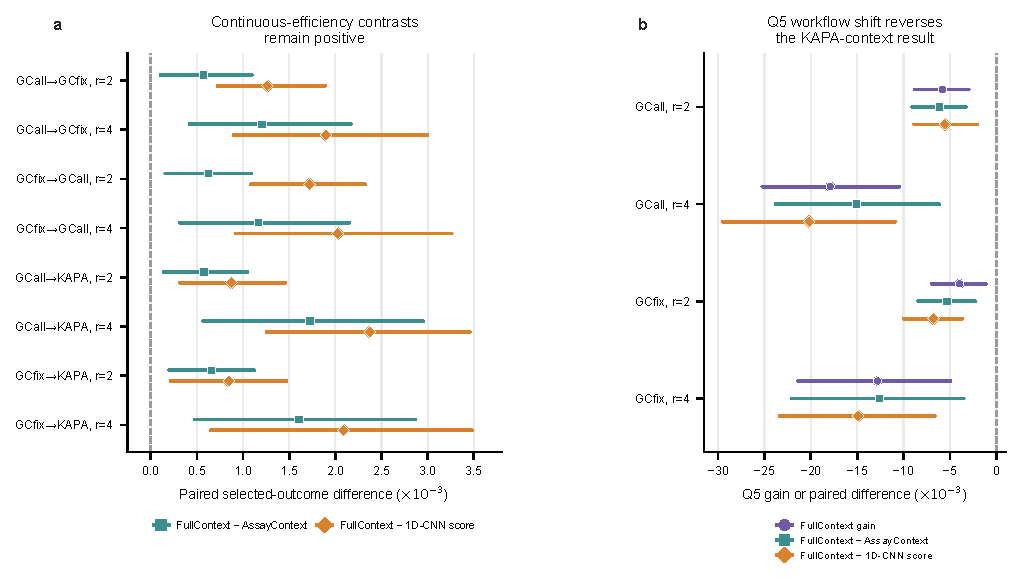
\includegraphics[width=\linewidth]{figures/paired_two_stage_sensitivity.pdf}
\caption{\textbf{Paired two-stage contrasts and the Q5 workflow-shift boundary.} (a) FullContext-minus-AssayContext and FullContext-minus-released-1D-CNN selected continuous-efficiency contrasts on the retrospective cross-pool and dated-plan external KAPA codebooks. (b) FullContext gain and its paired contrasts with AssayContext and the released 1D-CNN score in the secondary exploratory Q5 codebook. Points are bootstrap means and whiskers are percentile 95\% intervals from 2,000 corrected grouped-source plus target-fiber replicates; released CNN scores remained fixed. Intervals condition on published sequence-level outcomes and do not propagate technical-replicate, batch, normalization or assay-measurement uncertainty. The fiber is the target resampling unit. Source data accompany the figure.}
\label{fig:s-paired-two-stage}
\end{figure}

\begin{table}[H]
\centering
\small
\begin{tabular}{llrr}
\toprule
Direction & $r$ & FullContext range (s.d.) & FullContext-minus-AssayContext range (s.d.) \\
\midrule
GCall$\rightarrow$GCfix & 2 & 0.199--0.230--0.267 & 0.012--0.043--0.099 \\
GCall$\rightarrow$GCfix & 4 & 0.251--0.324--0.385 & 0.034--0.104--0.195 \\
GCfix$\rightarrow$GCall & 2 & 0.246--0.282--0.317 & 0.041--0.074--0.119 \\
GCfix$\rightarrow$GCall & 4 & 0.348--0.384--0.490 & 0.040--0.134--0.190 \\
\bottomrule
\end{tabular}
\caption{Sensitivity across 32 outcome-blind cross-pool library mappings. All displayed ranges are positive. They are deterministic mapping sensitivity, not confidence intervals or biological repeats.}
\label{tab:s-mapping-sensitivity}
\end{table}

The external KAPA mapping fixed by the dated local analysis plan remained the primary analysis. Across 32 additional post hoc outcome-blind mappings, FullContext gain, FullContext-minus-AssayContext and FullContext-minus-CNN were positive in all 32 settings for each source model and candidate width (Table~\ref{tab:s-external-mapping-sensitivity}). The primary mapping was reproduced from the frozen 2,053-row derived input table to numerical precision before these mappings were evaluated.

\begin{table}[H]
\centering
\scriptsize
\begin{tabular}{llrrr}
\toprule
Source & $r$ & FullContext gain & FullContext-minus-AssayContext & FullContext-minus-CNN \\
\midrule
GCall & 2 & 2.441--2.655--2.988 & 0.477--0.801--1.341 & 0.761--1.136--1.566 \\
GCall & 4 & 2.854--3.785--4.401 & 0.193--1.327--2.128 & 0.975--2.051--3.137 \\
GCfix & 2 & 2.332--2.534--2.910 & 0.453--0.808--1.387 & 0.680--1.043--1.520 \\
GCfix & 4 & 2.959--3.533--4.124 & 0.740--1.425--2.170 & 0.970--1.921--3.703 \\
\bottomrule
\end{tabular}
\caption{Post hoc external KAPA mapping sensitivity across 32 additional outcome-blind namespaces. Entries are deterministic min--median--max values in units of $10^{-3}$ measured efficiency; every displayed metric was positive in 32/32 mappings. These mappings are not confidence intervals or biological repeats, and they do not replace the dated-plan primary mapping.}
\label{tab:s-external-mapping-sensitivity}
\end{table}

\begin{table}[H]
\centering
\scriptsize
\begin{tabular}{llrrr}
\toprule
Mapping scope/source & $r$ & Mappings & Negative-fiber fraction min--median--max & Score variance min--median--max\\
\midrule
GCall$\rightarrow$GCfix & 2 & 32 & 0.271--0.312--0.346 & $4.49$--$5.09$--$5.57\times10^{-6}$\\
GCall$\rightarrow$GCfix & 4 & 32 & 0.125--0.195--0.258 & $5.56$--$6.34$--$6.76\times10^{-6}$\\
GCfix$\rightarrow$GCall & 2 & 32 & 0.260--0.300--0.326 & $5.84$--$6.87$--$7.30\times10^{-6}$\\
GCfix$\rightarrow$GCall & 4 & 32 & 0.148--0.203--0.258 & $7.34$--$8.62$--$8.91\times10^{-6}$\\
External KAPA, GCall source & 2 & 32 & 0.254--0.296--0.326 & $4.65$--$4.82$--$5.04\times10^{-6}$\\
External KAPA, GCall source & 4 & 32 & 0.133--0.180--0.258 & $5.91$--$6.02$--$6.10\times10^{-6}$\\
External KAPA, GCfix source & 2 & 32 & 0.264--0.305--0.338 & $5.21$--$5.39$--$5.56\times10^{-6}$\\
External KAPA, GCfix source & 4 & 32 & 0.172--0.211--0.289 & $6.57$--$6.72$--$6.82\times10^{-6}$\\
\bottomrule
\end{tabular}
\caption{Empirical FullContext fiber composition across outcome-blind mappings. Fractions and variances are descriptive properties of each grouping; they are neither confidence intervals nor biological replicates. Theoretical bijectivity of the rank map does not imply these empirical ranges.}
\label{tab:s-mapping-fiber-diagnostics}
\end{table}

Within-fiber random-choice tests used $B=100{,}000$ Monte Carlo draws and $P=(b+1)/(B+1)$. For each of the eight cross-pool/external-KAPA FullContext tests, $b=0$, so $P=1/100{,}001=9.9999\times10^{-6}$ was the minimum attainable value, not an exact analytic tail probability. Exact outputs for every selector are supplied in \texttt{fixed\_model\_randomization\_tests.tsv}; no star annotation or multiplicity claim is based on these values.

\section{Generated-language rate and correctness}

The 213-bit base domain has rate 1.972222 bits per variable-region nucleotide. Table~\ref{tab:s-generated} reports the complete $r=0,\ldots,6$ rate--score sweep. Five hundred and twelve deterministic payloads were tested for every $r$; the payload set included boundary values and SHA-256-derived ranks. Across the resulting 65,024 candidate checks, every sequence had length 108, GC count 49--59 and maximum homopolymer 3, and every physical rank, inverse modulo-$N$ rank, choice index and payload round-tripped. There were no duplicate logical candidates within a setting. Wrong length, ambiguous N, constraint violations, non-finite scores and inverse images with $q\geq2^{213}$ were rejected by their declared interfaces. A valid noncanonical fiber member was accepted by the payload decoder and rejected only by the optional canonical verifier; replacing the scorer did not alter payload recovery.

\begin{table}[H]
\centering
\small
\begin{tabular}{lrrrrrr}
\toprule
Selector source & $r$ & Candidates & Payload bits & Rate & Predicted mean gain & Predicted median gain \\
\midrule
GCall & 0 & 1 & 213 & 1.972222 & 0 & 0 \\
GCall & 1 & 2 & 212 & 1.962963 & 0.001343 & 0.001036 \\
GCall & 2 & 4 & 211 & 1.953704 & 0.002393 & 0.002198 \\
GCall & 3 & 8 & 210 & 1.944444 & 0.003091 & 0.002967 \\
GCall & 4 & 16 & 209 & 1.935185 & 0.003642 & 0.003625 \\
GCall & 5 & 32 & 208 & 1.925926 & 0.004229 & 0.004189 \\
GCall & 6 & 64 & 207 & 1.916667 & 0.004720 & 0.004692 \\
GCfix & 0 & 1 & 213 & 1.972222 & 0 & 0 \\
GCfix & 1 & 2 & 212 & 1.962963 & 0.001438 & 0.001156 \\
GCfix & 2 & 4 & 211 & 1.953704 & 0.002592 & 0.002448 \\
GCfix & 3 & 8 & 210 & 1.944444 & 0.003356 & 0.003163 \\
GCfix & 4 & 16 & 209 & 1.935185 & 0.003953 & 0.003907 \\
GCfix & 5 & 32 & 208 & 1.925926 & 0.004585 & 0.004502 \\
GCfix & 6 & 64 & 207 & 1.916667 & 0.005098 & 0.005048 \\
\bottomrule
\end{tabular}
\caption{Generated-language rate--score audit for 512 deterministic payload fibers per row. Rate is $(213-r)/108$ and excludes fixed adapters. Gain is selected FullContext score minus its candidate-fiber mean. Nonnegative own-model gain follows from maximization and is not biological evidence; all values are predictions on unmeasured sequences. Per-fiber minima, maxima, score variance, opposite-model evaluations and computation costs are machine-readable.}
\label{tab:s-generated}
\end{table}

The reduced length-8 codec, with GC count 3--5 and maximum homopolymer 3, contained 45,128 words by both dynamic programming and explicit enumeration. Every one of its 45,128 ranks was enumerated, unranked and reranked with zero failure. This all-rank test independently checks the implementation pattern at a tractable size; it is not a statistical sample of the 108-nt language.

Rank dispersion was inspected positionally rather than inferred from feature ranges. The modulo-$N$ candidates had first-base frequencies A 0.249575, C 0.249884, G 0.250302 and T 0.250240; over all 108 positions, each nucleotide frequency lay between 0.236868 and 0.261794. By contrast, a hypothetical modulo-$2^{213}$ lexicographic-prefix map would have first-base fractions A 0.408706, C 0.408706, G 0.182589 and T 0. Eight independently derived modulo-$N$ namespaces, each evaluated on 128 payloads at $r=2$ and $r=4$, had positive own- and cross-model gains and zero round-trip failures (Table~\ref{tab:s-generated-mappings}).

\begin{table}[H]
\centering
\small
\begin{tabular}{llrrr}
\toprule
Selector source & $r$ & Own gain min--median--max & Other-model gain min--median--max & Positive namespaces \\
\midrule
GCall & 2 & 0.002218--0.002308--0.002557 & 0.002258--0.002411--0.002691 & 8/8 \\
GCall & 4 & 0.003661--0.003731--0.003864 & 0.003736--0.003878--0.004045 & 8/8 \\
GCfix & 2 & 0.002351--0.002481--0.002774 & 0.002111--0.002212--0.002464 & 8/8 \\
GCfix & 4 & 0.003910--0.004020--0.004177 & 0.003474--0.003602--0.003722 & 8/8 \\
\bottomrule
\end{tabular}
\caption{Generated-score sensitivity across eight full-language affine namespaces. Ranges are algorithmic sensitivity, not confidence intervals or biological repeats; all 4,096 namespace-specific selected-sequence round trips passed.}
\label{tab:s-generated-mappings}
\end{table}

Generated-feature distribution was compared with both the complete source pool and its codec-eligible subset. For active FullContext features, maximum absolute standardized mean difference relative to the eligible subset was 0.038512 for GCall and 0.028609 for GCfix; minimum coverage inside source 1--99\% quantiles was 0.956270 and 0.955171, respectively. Maximum KS statistics were 0.226051 and 0.126193. Against the complete source pools, maximum absolute standardized mean difference reached 1.584 because generated sequences obey the explicit homopolymer and GC constraints while many source sequences do not. Quantiles, KS statistics and Wasserstein distances for every feature are supplied in \texttt{generated\_feature\_overlap.tsv}. These diagnostics describe computational domain shift and do not calibrate generated-sequence PCR outcomes.

\subsection{Single-edit, silent-misdecode and CRC composition boundary}

Choice fibers are a shaping layer and do not by themselves provide channel-error correction or integrity. To make this boundary executable, we formed 32 deterministic CRC-valid messages for each source-trained FullContext selector. Each logical payload comprised 195 message bits, a 16-bit CRC-16/CCITT-FALSE value (polynomial 0x1021, initial value 0xffff, no reflection or final xor) and two choice bits, totaling the 213-bit logical domain. The CRC was evaluated on the fixed 25-byte big-endian representation of the 195-bit message, including its leading zero padding. The standard ASCII check vector \texttt{123456789} returned 0x29b1.

For the 64 emitted $r=2$ codewords, we enumerated every single substitution (324), insertion (436) and deletion (108) operation per codeword, totaling 55,552 edit operations. All insertions and deletions were rejected by the fixed-length interface. Among substitutions, 12,093 operations passed the base decoder with a payload different from the transmitted payload. CRC-16 detected every such wrong-payload acceptance in this deterministic sample; this observed zero is not a proof for arbitrary multi-edit channels. The optional canonical verifier alone left 8,142 wrong-payload acceptances, confirming that canonicality is not an integrity check (Table~\ref{tab:s-channel-boundary}).

\begin{table}[H]
\centering
\scriptsize
\begin{tabular}{llrrrrrr}
\toprule
Selector & Edit & Operations & Length reject & Constraint reject & $q\geq M$ reject & Wrong payload & CRC residual \\
\midrule
GCall & substitution & 10,368 & 0 & 666 & 3,656 & 6,046 & 0 \\
GCall & insertion & 13,952 & 13,952 & 0 & 0 & 0 & 0 \\
GCall & deletion & 3,456 & 3,456 & 0 & 0 & 0 & 0 \\
GCfix & substitution & 10,368 & 0 & 654 & 3,667 & 6,047 & 0 \\
GCfix & insertion & 13,952 & 13,952 & 0 & 0 & 0 & 0 \\
GCfix & deletion & 3,456 & 3,456 & 0 & 0 & 0 & 0 \\
\bottomrule
\end{tabular}
\caption{Deterministic single-edit boundary audit. Counts are edit operations, not independent molecules or stochastic channel draws. CRC residual denotes a wrong decoded payload that also passed CRC-16. The audit demonstrates composition with an integrity layer, not correction, dropout handling, clustering, consensus, sequencing recovery or file recovery.}
\label{tab:s-channel-boundary}
\end{table}

Adding the CRC reduced the retained user message from 211 to 195 bits at $r=2$, or 1.80556 message bits per 108-nt variable region. No outer error-correcting code was implemented or benchmarked. Machine-readable emitted codewords, all edit outcomes, summary counts, reference vectors, environment metadata and hashes are in \path{channel_error_boundary}.

\section{Complexity and machine-specific runtime}

For length $n$, whole-sequence GC-count range $G$ and homopolymer bound $h$, the exact completion table has $O(nG|\DNA|h)$ reachable state slots and at most $|\DNA|$ transitions per state. Once cached, exact rank and unrank make $O(n|\DNA|)$ branch-mass queries. For a score with evaluation cost $S(n)$, choice encoding evaluates $2^r$ candidates and therefore costs $O(2^r[n|\DNA|+S(n)])$. Payload decoding reranks one sequence, inverts one modular affine map over $N$, checks $q<M$ and shifts $r$ bits, so it remains $O(n|\DNA|)$ and does not evaluate the score. The FullContext feature implementation constructs reverse-complement anti-diagonal tables for the variable and full constructs and has $S(n)=O(n^2)$ time and memory.

The benchmark used one process, 128 fixed payloads per choice setting, three repeats and 4,096 base ranks. It was run on the recorded Intel macOS host with Python 3.12.13. All timed operations retained exact round trips (Table~\ref{tab:s-runtime}).

\begin{table}[H]
\centering
\small
\begin{tabular}{lrrrr}
\toprule
Operation & $r$ & Candidates & Items & Median ms/item \\
\midrule
Base unrank & 0 & 1 & 4,096 & 0.928 \\
Base rank & 0 & 1 & 4,096 & 0.841 \\
FullContext choice encode & 0 & 1 & 128 & 8.577 \\
FullContext choice encode & 2 & 4 & 128 & 42.592 \\
FullContext choice encode & 4 & 16 & 128 & 154.996 \\
Payload decode & 0 & 1 & 128 & 0.915 \\
Payload decode & 2 & 4 & 128 & 0.975 \\
Payload decode & 4 & 16 & 128 & 1.022 \\
\bottomrule
\end{tabular}
\caption{Single-process implementation timing. Cold completion-table construction took 0.432 s and produced 41,101 cache entries; peak process high-water memory was 142.2 MiB. Values are machine-specific measurements from the modulo-$N$ implementation, not biological replicates or an end-to-end storage comparison.}
\label{tab:s-runtime}
\end{table}

\section{Prior art and novelty matrix}

The novelty claim is deliberately narrower than constrained coding, shaping/list-selection, candidate screening or sequence optimization alone (Table~\ref{tab:s-comparators}). The present numerical benchmark is not limited to this scope table: the released Gimpel 1D-CNN outputs and hard rule were run on identical experimental fibers in Tables~\ref{tab:s-public-sota} and \ref{tab:s-external-sota}.

\begin{table}[H]
\centering
\scriptsize
\begin{tabular}{>{\raggedright\arraybackslash}p{0.16\linewidth}>{\raggedright\arraybackslash}p{0.22\linewidth}>{\raggedright\arraybackslash}p{0.24\linewidth}>{\raggedright\arraybackslash}p{0.28\linewidth}}
\toprule
Work or family & Established contribution & Relationship to candidate choice & Boundary relative to this study \\
\midrule
Enumerative and sliding-block coding \cite{cover1973enumerative,adler1983slidingblock} & Exact constrained indexing and finite-state coding & Defines reversible base maps, not an assay-trained representative selector & Establishes the rank/unrank and constrained-coding foundations. \\
Trellis shaping \cite{forney1992trellisshaping} & Selects a low-cost representative from an equivalence class while preserving data semantics & Direct precedent for representative selection with recoverable information & Removes any claim that equivalence-class selection is itself new. \\
List-encoding CCDM \cite{wu2022listccdm} & Produces semantically equivalent candidate sequences and selects by an auxiliary metric & Direct precedent for list generation followed by metric-based selection & Establishes list-selection/shaping prior art outside oligonucleotide assays. \\
GC/homopolymer block codes \cite{wang2019bioconstrained,immink2019balancedhomopolymer} & Reversible biochemical constraint control & May provide valid codewords without an arbitrary assay utility & Removes any broad novelty claim for exact GC/homopolymer coding. \\
Explorer \cite{dou2024explorer} & De Bruijn-graph coding under local and global biochemical constraints & Expands exact constrained-code design beyond the present simple GC/run language & Does not report payload-indexed fixed fibers selected by a replaceable empirical PCR scorer. \\
DNA Fountain \cite{erlich2017dnafountain} & Seed generation and screening in a storage architecture & Chooses acceptable droplets by screening candidates & Establishes stochastic candidate screening; its rate/failure contract differs from fixed fibers. \\
DNA Chisel \cite{zulkower2020dnachisel} & Extensible optimization under sequence specifications & Optimizes a sequence under composable objectives & Does not by itself define the present fixed-payload fiber inverse. \\
RNAblueprint \cite{hammer2017rnablueprint} & Uniform constrained nucleic-acid sampling & Samples candidates compatible with structural targets & Addresses sequence design rather than payload-indexed assay choice. \\
DNA-Aeon \cite{welzel2023dnaaeon} & Arithmetic coding, constraints and error correction & Supports reversible storage coding and custom constraints & Establishes strong codec prior art; no source-trained PCR selector on these fibers is reported. \\
SCONE \cite{ruan2026scone} & Constraint-aware arithmetic coding for learned latents & Adapts coding probabilities to biochemical constraints & Establishes a reversible learned-codec interface; no present fixed-fiber PCR evaluation is reported. \\
HEDGES and Composite Hedges Nanopores \cite{press2020hedges,zhao2024compositehedges} & Indel-aware inner coding and nanopore-oriented codec/recovery pipelines & Protect information against channel errors rather than selecting an assay-ranked representative & Establish that the present noiseless shaping layer requires separate integrity and error-correction components. \\
FrameD \cite{volkel2023framed} & Modular DNA-storage simulation, error injection and pipeline comparison & Provides system-level verification infrastructure & Addresses end-to-end design evaluation rather than the present fixed-fiber semantic interface. \\
Recent codec benchmark and Gungnir \cite{gimpel2026codecbenchmark,zhang2026gungnir} & Standardized codec benchmarking and high-error-tolerance recovery & Quantify substitution/indel/dropout tolerance with inner/outer or search-based protection & Define current channel-code practice; the present work neither competes on recovery nor claims error correction. \\
Gimpel 1D-CNN/filter \cite{gimpel2025pcrbias} & PCR-efficiency prediction and filter validation & Supplies assay-trained rankings and the published hard rule & Used here as the numerical external comparator on identical public fibers. \\
\bottomrule
\end{tabular}
\caption{Prior-art and novelty matrix. Choice fibers instantiate a fixed-rate shaping/list-selection interface for an exact constrained oligonucleotide codec. The supported increment is its assay-trained use, score-independent payload inversion, full-language rank dispersion, strict $r$-bit cost and retrospective PCR evaluation. The table does not claim technical inferiority of cited methods.}
\label{tab:s-comparators}
\end{table}

\begin{table}[H]
\centering
\scriptsize
\resizebox{\linewidth}{!}{%
\begin{tabular}{lcccccccc}
\toprule
Method family & Exact payload inverse & Fixed candidates/payload & Fixed rate loss & Decoder score-free & Scorer can change & Global totality & Arbitrary deterministic score & Real PCR evaluation\\
\midrule
Enumerative constrained coding & Yes & Not intrinsic & Yes & Not applicable & Not applicable & Yes on declared domain & No interface by itself & No\\
Explorer / constrained graph coding & Yes on declared code & Not intrinsic & Fixed by construction & Yes & Not intrinsic & Method/domain-dependent & Constraint objective & No PCR-selection test\\
Rejection sampling / DNA Fountain screening & Architecture-dependent & Usually capped/variable & Variable/effective & Usually & Usually & Not under a finite cap & Predicate/metric-dependent & Method-dependent\\
Trellis shaping / list encoding & Yes & Method-dependent & Often fixed & Often & Often & Method-dependent & Auxiliary metric-dependent & Not in cited oligo PCR setting\\
Distribution matching & Yes & Method-dependent & Fixed or asymptotic & Yes & Method-dependent & Domain-dependent & Not necessarily & No\\
Heuristic motif filtering / reranking & Not by itself & Variable & Variable & Not by itself & Yes & No general guarantee & Objective-dependent & Sometimes\\
Model-based sequence design & Not by itself & Variable & Variable & Often model-dependent & Yes & No general guarantee & Model-specific & Method-dependent\\
Constrained codebook search & Codebook-dependent & Codebook-dependent & Codebook-dependent & Codebook-dependent & Codebook-dependent & Finite codebook only & Search-dependent & Method-dependent\\
HEDGES / channel-code systems & Yes with declared stack & Not the interface & Redundancy-dependent & Yes & Not applicable & Channel/domain-dependent & No arbitrary assay interface & Method-dependent\\
Present choice fibers & Yes & Exactly $2^r$ & Exactly $r$ bits & Yes & Yes; history decodes & Yes on declared domain & Yes, if deterministic/finite & Retrospective measured PCR\\
\bottomrule
\end{tabular}}
\caption{Property-level conceptual comparison requested for novelty positioning. Entries summarize method-family contracts rather than asserting that every implementation in a family has the same property. The present contribution is the joint contract in the last row and its retrospective PCR evaluation, not the individual ingredients.}
\label{tab:s-property-matrix}
\end{table}

\section{Matched baselines and totality}

Composition, AssayContext and FullContext selectors used identical fibers, so model differences cannot be attributed to different candidate sets. The $r=0$ condition is the no-choice control. A second comparator used the source pool's top-quartile FullContext threshold and inspected at most the same $2^r$ candidates. It failed if no candidate crossed the threshold, whereas fixed choice always emitted the within-fiber maximizer and retained a defined payload inverse.

\begin{table}[H]
\centering
\small
\begin{tabular}{lrrrr}
\toprule
Threshold source & $r=0$ & $r=2$ & $r=4$ & $r=6$ \\
\midrule
GCall FullContext & 0.7637 & 0.3281 & 0.0137 & 0.0000 \\
GCfix FullContext & 0.7383 & 0.2891 & 0.0059 & 0.0000 \\
Fixed-choice codec & 0 & 0 & 0 & 0 \\
\bottomrule
\end{tabular}
\caption{Payload failure fraction for threshold rejection among 512 deterministic generated payloads per setting. Zero sampled threshold failures at $r=6$ is not a theorem; fixed choice is total because it does not require a threshold crossing.}
\label{tab:s-threshold}
\end{table}

The threshold experiment transfers a public-source score cutoff to generated sequences and is therefore a computational comparator, not a biological failure-rate estimate. Its purpose is to separate a fixed-cardinality, fixed-rate map from rejection whose success depends on the score distribution.

\section{Negative domain boundary in DT4DDS}

The DT4DDS replay used 12,472 Genscript and 12,000 Twist public reference sequences from a synthesis--aging--PCR--sequencing workflow \cite{gimpel2023digitaltwin}. Supplier pools were analysed separately. Mean $\log_2(\mathrm{CPM}+1)$ and day-7 minus mean-day-0 $\log_2(\mathrm{CPM}+1)$ are composite detectability endpoints, not isolated molecular survival or recovery.

\begin{table}[H]
\centering
\small
\begin{tabular}{llrr}
\toprule
Pool & Endpoint & $\Delta$ OOF Spearman & Paired 95\% interval \\
\midrule
Genscript & Mean normalized abundance & $-0.000325$ & [$-0.001464$, 0.000879] \\
Twist & Mean normalized abundance & $-0.001381$ & [$-0.003593$, 0.000810] \\
Genscript & Day-7 change & 0.000092 & [$-0.000413$, 0.000599] \\
Twist & Day-7 change & $-0.000430$ & [$-0.001015$, 0.000167] \\
\bottomrule
\end{tabular}
\caption{Increment from adding variable-region $W$ to composition, candidate count and longest stem. Every interval includes zero.}
\label{tab:s-dt4dds}
\end{table}

The controlling nested result is null. Earlier univariate associations are not used to label $W$ a universal molecular-risk direction. No DT4DDS sequence was generated by the present choice codec, and assigned-read abundance cannot establish file recovery.

\section{Reproducibility inventory}

The anonymous bundle exposes two separate entry points:
\begin{verbatim}
./reproduce_from_frozen_outputs.sh
./reproduce_from_public_inputs.sh
\end{verbatim}
The frozen-output runner verifies package and nested manifests, recomputes the external mapping-sensitivity and major-revision diagnostic summaries from frozen derived tables, regenerates all three figures, reruns manuscript consistency checks and compiles both anonymous PDFs. The public-input runner verifies the required upstream hashes, reports missing inputs with their expected locations and invokes the full project-layout workflow when those inputs are present. Both use an explicitly supplied compatible \texttt{PYTHON} or an exact-version environment outside the package; neither modifies a system or base environment.

The \path{reversible_choice_codec} output directory contains exact-language, modulo-$N$ generated-code, positional-composition, feature-domain and mapping-namespace outputs. The \path{sota_and_external_validation} directory contains input audits, source coefficients, identical-fiber benchmark summaries and distributions, endpoint-matched event tables, Q5 sensitivity, pairwise comparisons, randomization tests, 2,000 corrected grouped-source two-stage bootstrap replicates and provenance. The \path{channel_error_boundary} directory contains the CRC-protected emitted codewords, all 55,552 single-edit outcomes, summary counts, reference vector, environment and manifest. The external mapping-sensitivity directory contains the frozen derived input table, all 32 mappings, descriptive summaries and a primary-mapping reproduction check. The \path{major_revision_diagnostics} directory contains the dataset-partition and evidence-hierarchy tables, negative-fiber and post hoc feature-stratification summaries, score-margin abstention sensitivity, $r=0,\ldots,6$ rate--benefit diagnostics, score-determinism audit, decoder failure contract and leakage-scope table. The shared deterministic-selection helper implements the declared 12-decimal integer key and smallest-choice-index tie rule. Full source--external and source--source sequence-independence audits and the machine-specific timing snapshot are stored in separate manifest-locked directories. The public-input acquisition helper downloads or checks out third-party files at pinned hashes/commits; those inputs retain their upstream terms and are not relicensed by this project.

The recorded run used Python 3.12.13, NumPy 2.5.0, pandas 3.0.3, SciPy 1.18.0, scikit-learn 1.9.0 and joblib 1.5.3 on macOS 13.7.8. Randomized operations have explicit integer seeds or SHA-256 namespaces. Code and frozen derived outputs are public at \url{https://github.com/nessajzhang/exact-reversible-choice-coding} under the BSD-3-Clause licence. A persistent archive URL or identifier and contact metadata remain author-controlled submission fields; no creator identity is inferred in this anonymous version.

\begingroup
\small
\bibliographystyle{plain}
\bibliography{references}
\endgroup

\end{document}
